\chapter{Grundlagen} \label{chapter_2}
Für ein besseres Verständnis und genauere Definition wird das Produkt zu Beginn beschrieben. Darauf aufbauend wird der Einsatz von Produktkonfiguratoren in diesem Segment behandelt. Mobile Anwendungen stellen die dritte Grundlage für diese Arbeit.

\section{Definition Produkt}
Im Marketing wird ein Produkt als Ergebnis im Produktionsprozess definiert. Innerhalb des Prozesses entsteht ein Produkt, welches am Ende eine Summe mehrerer materieller oder immaterieller Eigenschaften besitzt \cite{bib:product}. Aus Sicht des Kunden ist ein solches Produkt ein Einzelstück, das für die Befriedigung eines Nutzens eingesetzt werden kann. Ein konkretes Produkt ist bspw. ein Auto, da es ein Resultat eines Produktionsprozesses ist. Ein Kunde nimmt das Produkt als einzelnes Objekt wahr. Bei der Produktion hingegen ist das Auto eine Zusammenstellung aus mehreren Einzelteilen. Hier besteht ein Auto aus den vier Hauptbereichen Karosserie, Motor, Innenausstattung und Getriebe. Die Innenausstattung besteht wiederum aus Sitzen und Armaturen. Diese Verfeinerung ist die Basis für die Individualität eines bestimmten Produktes. Je mehr Verfeinerungen existieren, desto komplexer ist ein einzelnes Produkt. Sobald der Hersteller mehr als eine Variante einer Einzelkomponente für den Kunden zur Verfügung stellt, lässt sich ein Produkt individualisieren. Für die Durchführung einer Individualisierung gibt es verschiedene Möglichkeiten. Die Einzelfertigung fertigt immer nur eine Einheit eines Produktes, wodurch jedes Produkt individuell ist. Das Gegenstück hierzu ist die Massenproduktion, bei der große Mengen des gleichen Produktes, mit unterschiedlichen Bauteilen hergestellt werden. Zwischen diesen beiden Extremen liegt die sogenannte mass-customization. Bei diesem Ansatz werden Produkte meist in Bausteine unterteilt, die vom Kunden individuelle zusammengestellt werden können. Am Ende entsteht das Produkt.
 \par 

Voraussetzung für die Individualisierung ist eine veränderte Wahrnehmung des Kunden. Ein Produkt darf nicht mehr als einzelnes Objekt gesehen werden. Für die individuellen Anpassungen muss der Kunde ein Produkt als eine Zusammenstellung mehrerer Komponenten verstehen. Diese veränderte Wahrnehmung muss dem Kunden vermittelt werden, um ihm dadurch eine Individualisierung seines Produktes zu ermöglichen. \par

Die zweite große Herausforderung entsteht bei baulichen Abhängigkeiten der einzelnen Produktteile. Bei einem komplexen Produkt mit vielen Einzelteilen können viele Abhängigkeiten entstehen. Wenn bei einem Auto bspw. ein bestimmter Motor ausgewählt wurde, so lassen sich nur für den Motor passende Getriebe einbauen. Durch die Verwendung mehrerer Möglichkeiten für eine bestimmte Einzelkomponente steigt ebenfalls die Anzahl der Abhängigkeiten. Die Prüfung dieser Abhängigkeiten muss ein Experte durchführen, der sich bestens mit der Produktzusammensetzung auskennt. Damit die einzelnen Vorgänge nicht zu komplex werden, sind geeignete Formen der Darstellung nötig.

\subsection{Produktkatalog}
Um dem Kunden einen Einblick in ein Produkt zu verschaffen werden sogenannte Produktkataloge verwendet. Diese Kataloge sind meist in Papierform vorhanden und enthalten für den Kunden relevante Informationen über ein Produkt.  Hierbei wird oben genanntes Ziel, beim Kunden eine andere Sicht des Produktes zu erzeugen, verfolgt. Für das Erreichen dieses Ziels bestehen Produktkataloge aus anschaulichen Bildern und besitzen eine übersichtliche Struktur für ein schnelles Finden des gewünschten Produktes. Die Herausforderung bei einem Katalog besteht bei der Abwägung, wie viele technische Informationen enthalten sein müssen, damit ein Produkt für den Kunden konfigurierbar wird. Je weniger der Kunde von der technischen Seite wissen muss, desto einfacher gestaltet sich der gesamte Konfigurationsprozess.  


\subsection{Boolesche Algebra in der Produktmodellierung}
Die Zweite bereits genannte Herausforderung bei Produkten ist das Auswerten bzw. Modellieren der  komplexen Abhängigkeiten von Einzelbauteilen.  Ein Ansatz zur Lösung dieses Problems ist die boolesche Algebra. Bei der booleschen Algebra werden zwei Werte: wahr und falsch definiert \cite{bib:boolescheAlgebra1}. In der Aussagenlogik wird dies so verwendet, dass eine Aussage, wie "'Heute regnet es"' entweder wahr oder falsch sein kann \cite{bib:boolescheAlgebra2}. Mithilfe von verschiedenen Operatoren lassen sich die Aussagen miteinander Verknüpfen, so dass auch komplexere Zusammenhänge möglich sind. Grundlegend zu nennen sind hier die Disjunktion (Symbol: $\vee$), bei der einer von zwei Aussagen wahr sein muss, um den kompletten Ausdruck wahr werden zu lassen. Bei der Konjunktion (Symbol: $\wedge$) müssen beide Aussagen zutreffend sein. Um Schlussfolgerungen durchführen zu können ist die sogenannte Wenn-Dann Verknüpfung (Symbol: $\Rightarrow$) wichtig. Der Ausdruck "'Wenn Aussage A, dann Aussage B"' ist falsch, wenn Aussage A richtig und B falsch ist. In allen weiteren Konstellationen ist der gesamte Ausdruck wahr. 
\par

Übertragen auf das Modellieren eines Produktes können die Abhängigkeiten der Einzelbauteile mithilfe der booleschen Algebra aufgezeigt werden. Eine Auswertung dieser Modellierung erzeugt eine klare Aussage über die technische Umsetzung der aktuellen Auswahl. Hierbei können komplexe Zusammenhänge innerhalb eines Produktes korrekt abgebildet werden. Für das Auto Beispiel wäre eine Regel für die Beziehung von Motor und Getriebe in folgender Form möglich: \par
\begin{center}
$ Verwendung von Motor A    \Rightarrow Einbau von Getriebe A $
\end{center} \par
Bedeutung: Wenn der Motor A verwendet werden soll, dann muss das Getriebe A eingebaut werden, damit die Regel zutrifft. Wenn der Motor A nicht eingebaut wird, ist für die Erfüllung dieser Regel der Einbau des Getriebes keine Voraussetzung. 
\par
Ein Problem, welches bei der Modellierung mit booleschen Regeln auftritt sind sogenannte Alternativen. Diese treten bei einer Zusammenstellung auf, bei der es mehrere Möglichkeiten gibt, wie eine Aussage wahr werden kann. Ein Beispiel wäre hier, dass die Auswahl des Armaturenbrett oder des Sitzes gefordert wird, wenn ein Motor und ein Getriebe ausgewählt wurde. Die Modellierung des Beispiels würde folgendermaßen aussehen: \par
\begin{center}
$ Motor A \wedge Getriebe A \wedge (Sitz A \vee Armaturenbrett B )  $
\end{center} \par
Damit diese Bedingung wahr werden kann, müssen entweder Sitz A oder Armaturenbrett B ausgewählt werden. Eine weitere Möglichkeit in diesem Fall wäre die Auswahl beider Komponenten. Dieser konkrete Fall würde beim Einbau von Motor A und Getriebe A somit drei Alternativen bieten. Dieses Problem bei der Produktkonfiguration mit booleschen Regeln gilt es zu beachten, sowie Möglichkeiten zu finden, wie diese ausgewertet werden können.

\section{Produktkonfiguratoren}\label{konfiguratoren}
Die Definition, welche Probleme bei einem komplexen Produkt auftreten können wurde im vorigen Abschnitt geklärt. Das Problem, wie eine große Anzahl der booleschen Regeln, die für die Produktmodellierung benötigt werden verarbeitet werden können bleibt bestehen. Eine Lösungsmöglichkeit bieten sogenannte Produktkonfiguratoren.
Das Ziel des Konfigurators ist es, produktspezifisches Wissen für die Anwender bereit zu stellen, welches zuvor von Experten in das System eingepflegt wird. Dieses hilft beim individuellen Zusammenstellung des Produktes durch die Verwendung des Produktwissens. Ein solches System wird in die Kategorie der Expertensysteme\cite{bib:puppe} oder wissensbasierte Systeme eingeordnet. Der Aufbau eines solches System ist in Abbildung \ref{expert_system_structure} zu sehen. \par
\begin{figure}
\centering
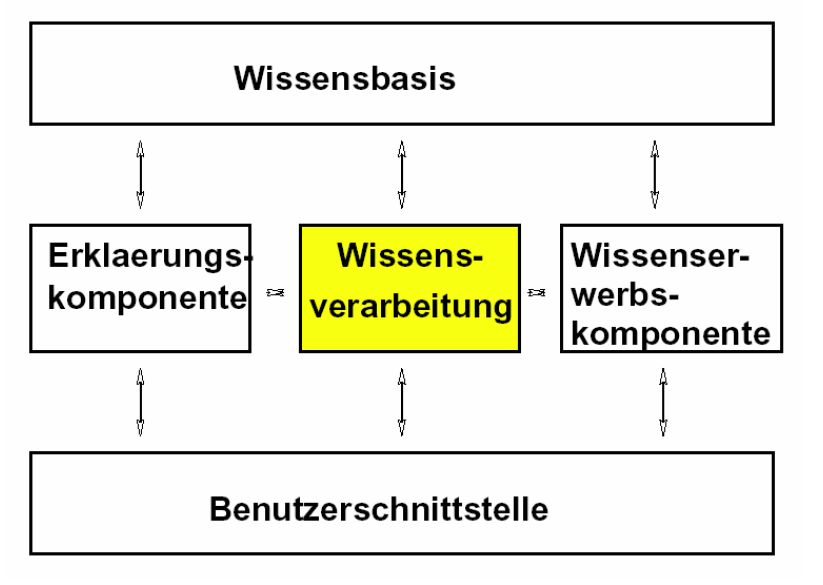
\includegraphics[width=250px]{images/expertensysteme}
\caption{Aufbau eines Expertensystems \cite[s.6]{bib:keller}}
\label{expert_system_structure}
\end{figure}

Die zentrale Komponente ist die \textit{Wissensverarbeitung}. Diese hat auf alle weiteren Komponenten Zugriff und interagiert mit diesen. Es werden die erhaltenen Fakten mithilfe der vorhandenen Regeln verknüpft. Aus der Verknüpfung werden neue Fakten gewonnen, die auf der \textit{Benutzerschnittstelle} angezeigt werden. Die Wissensbasis ist für das Speichern des Expertenwissens in Fakten und Regeln zuständig. Die Speicherung der Daten kann auf folgende zwei Arten geschehen\cite{bib:expert1}:\par
\begin{itemize}
        \item \textbf{generisch}: unabhängig vom aktuellen Anwendungsfall. Meist in einfachen Wenn-Dann-Regeln oder auf einem Modell beruhend. 
        \item \textbf{fallspezifisch}: stellt Lösungen für einen konkreten Anwendungsfall bereit.
\end{itemize}
 Die Pflege dieser Basis erfolgt durch die \textit{Wissenserwerbskomponente}. Mit deren Hilfe lässt sich das vorhandene Expertenwissen in das System einpflegen. Die \textit{Erklärungskomponente} unterstützt das Nachvollziehen des Ergebnisses durch Erläuterungen zu den getätigten Entscheidungen.

\subsection{CAS Configurator Merlin} \label{configurator}
Das Produkt CAS Configurator Merlin ist die Konfigurationslösung der CAS Software AG für große und mittelständische Unternehmen. Das Produkt besteht aus Standardkomponenten, die auf die einzelnen Bedürfnisse der Großkunden angepasst werden. In Abbildung \ref{airbus_structure} ist der Aufbau und das Zusammenspiel der verschiedenen Komponenten des Konfigurators zu sehen: \par
\begin{figure} [H]
\centering
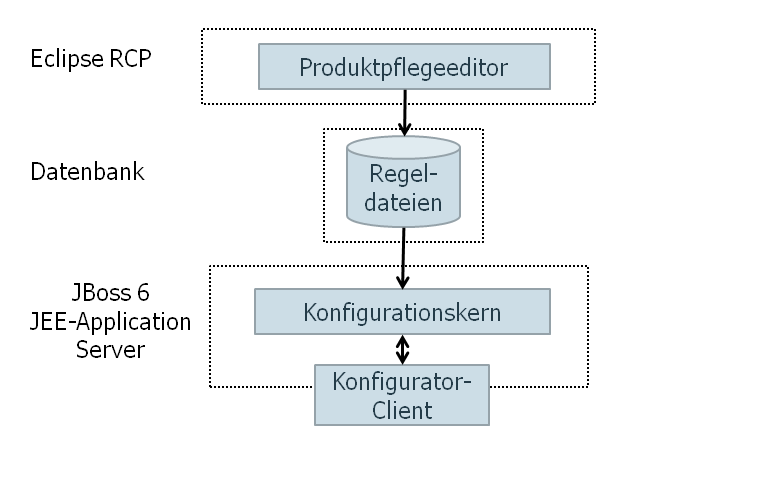
\includegraphics[width=\hsize]{images/AirbusAufbau}
\caption{Architektur und Datenfluss der Merlin Komponenten}
\label{airbus_structure}
\end{figure}
Die Wissensverarbeitungs-Komponente aus Abschnitt \ref{konfiguratoren} ist hier der sogenannte \textit{Konfigurationskern}. Der Kern wertet die zuvor zusammengestellten Produktkomponenten aus. Für die Auswertung verwendet er sogenannte Regeldateien, die mit dem \textit{Produktpflegeeditor} modelliert wurden. Diese Regeln sind auf booleschen Algebra aufgebaut um komplexe Abhängigkeiten der Einzelteile eines Produktes modellieren zu können. Die Speicherung dieser Dateien erfolgt in der \textit{Datenbank}.
\par
 Der Konfigurationskern berechnet ebenfalls sogenannte Alternativen. Diese treten auf, sobald die derzeitige Selektion alleine, ohne Hinzunahme von weiteren Bauteilen, nicht umsetzbar ist. Der Konfigurator kann in diesem Fall neue Möglichkeiten (Alternativen) vorschlagen, damit die Konfiguration durchgeführt werden kann. Die Auswahl der Konfigurationselemente erfolgt im sogenannten \textit{Konfigurator-Client}. Der Client ist mit der Benutzerschnittstelle im Expertensystem zu vergleichen. \par

Der Konfigurationskern, sowie der Client befinden sich auf einem Java-Application-Server. Der Produktpflegeeditor ist eine eigenständige Rich-Client Anwendung, welche auf dem Eclipse Rich-Client-Plattform Framework\cite{bib:eclipseRCP} basiert.

\subsection{Anwendungsbeispiel der Arbeit} \label{airbusConfigurator}
Damit die Arbeit an einem geeigneten Beispiel durchgeführt werden kann, wird der vorhandene Produktkonfigurator eines Flugzeugherstellers verwendet. Hier soll anhand des vorhandenen Prozesses gezeigt werden, wie eine Vereinfachung des gesamten Workflows bei einer Produktkonfiguration mit der Unterstützung einer mobilen Anwendung aussehen kann. \par 

Die aktuelle Konfigurationslösung wird für den Upgradeprozess eines vorhandenen Flugzeuges eingesetzt. Die Upgrades werden in die Kategorien Kabine und System eingeordnet. Alles was ein Flugzeugpassagier sehen kann, gehört in den Kabinenbereich. Alle weiteren Elemente sind Systemupgrades. Bei der Herstellung eines Flugzeuges wird derzeit hauptsächlich Einzelfertigung betrieben. Dies hat zur Folge, dass jedes Flugzeug sehr individuell ist. Aus diesem Grund ist die Konfiguration für ein Upgrade sehr aufwändig und komplex. Damit ein Upgrade möglich ist, werden Status definiert, die ein Flugzeug erreichen kann. Auf Basis dieser Status werden die möglichen Upgrades definiert. Der Konfigurationsraum ist von der jeweiligen Maschine abhängig und liegt bei 40 - 50 Möglichkeiten im Systembereich. Im Kabinenbereich ist ein komplettes Upgrade der Innenausstattung möglich. Deshalb sind hier ähnliche Möglichkeiten, wie bei der initialen Erstellung des Flugzeuges vorhanden.
\par


Dieses Anwendungsfeld ist besonders herausfordern, da somit zu der Auswahl der Produktkomponenten zusätzlich einzelne oder mehrere Flugzeuge ausgewählt werden müssen. Dies hat zur Folge, dass eine übersichtliche Darstellung der Upgrades alleine nicht ausreicht. Es muss ebenfalls eine Lösung für die Auswahl der einzelnen Flugzeuge gefunden werden.  Dadurch, dass jedes Flugzeug individuell zusammengestellt wurde, muss jedes auch eigenständig überprüft werden. 


\section{Mobile Anwendungen} \label{mobileAppsGrundlagen}
Die Frage, wie der Kunde besser an dem Entstehungsprozess eines Produktes teilhaben kann und dessen komplexen Aufbau verstehen kann ist nur über ausreichend Kommunikation und Wissensvermittlung zu bewerkstelligen. Eine Möglichkeit zur Unterstützung dieses Prozesses bieten mobile Anwendungen.\par

Diese sind definiert als eine Software, die auf einem Smartphone oder Tablet verwendet wird. Mit dieser Form der Anwendung sind neue Anwendungsgebiete in der Software möglich. Ein neues Einsatzgebiet ist der mobile Einsatz der App bei einem Kunden vor Ort \cite{bib:mobileMarketing}. Hier können insbesondere Tablet-PCs die Kommunikation mit dem Kunden fördern \cite{bib:tableVertrieb}. Die Vorteile durch den großen Bildschirm und die Möglichkeit wie bei einem Blatt Papier den Kunden ins Verkaufsgespräch mit einzubeziehen sind hier überzeugend. Eine Bedienung der Geräte durch Touch-Eingaben ermöglicht eine bessere Interaktion mit der Software. Die Möglichkeiten beim Einsatz dieser Geräte im Geschäftsumfeld ist noch nicht ausgeschöpft und birgt auch weiterhin Potenziale \cite[Fazit]{bib:mobileMarketing2}. In diesem Markt gilt es sich durch gute Anwendungskonzepte zu etablieren. \par

Für Entwickler einer mobilen Anwendung ist der Umgang mit den begrenzten Ressourcen auf dem Endgerät wichtig. 
Aufgrund der geringen Speicherkapazität der mobilen Geräte, sowie die Vermeidung von hohem Synchronisierungsaufwand ist eine Ablegung der Daten auf einem leistungsstärkeren Gerät essentiell. Deshalb ist eine Anbindung an einen Server eine wichtige Grundvoraussetzung bei einer mobilen Anwendung, wenn viele Daten zu verarbeiten sind.  Durch die immer bessere mobile Anbindung an das Internet wird die Verbindung mit einem entfernten System einfacher. Bei der Entwicklung einer mobilen App ist damit die Entscheidung über die Online und Offline Komponenten wichtig.
Ebenfalls von einer großen Bedeutung ist die Auswahl der richtigen Art der Anwendung. Hier stehen drei Möglichkeiten zur Verfügung, die aufgrund von unterschiedlichen Einschränkungen verschiedene Ziele verfolgen. Im Folgenden werden diese drei Arten vorgestellt.

\subsection{Native Anwendungen}
Native Anwendungen sind auf die jeweilige Zielplattform beschränkt \cite{bib:mobilePlattform}. Die Anwendung kann nur auf dem gewählten Betriebssystem ausgeführt werden. Die Programme für native Apps werden dafür mithilfe des vorgegebenen Frameworks entwickelt. Die Verbreitung dieser Anwendungen auf die Endgeräte der einzelnen Benutzer erfolgt über spezielles Software-Stores. Diese Stores werden von den Herstellern der jeweiligen Betriebssysteme bereitgestellt. Die zentrale Verwaltung der Apps sorgt für ein schnelles Verbreiten der Anwendung. \par

 Die Vorteile einer nativen Anwendung liegen im Bereich der Performance und der Funktionen. Da die Programmierung der gegebenen Hardware angepasst wird, sind native Anwendungen für das Zielsystem optimiert. Durch die Optimierung können die Hardwareressourcen besser ausgenutzt werden. Die zweite Stärke von diesem Anwendungstyp ist der erweiterte Funktionsumfang \cite{bib:nativeBS2}. Es können lokale Datenbanken, 3D-Renderer, lokale Sensoren und Ressourcenmanager der Plattform ohne Anpassungen verwendet werden. Dies erhöht die Anzahl der Möglichkeiten, die mit einer nativen Anwendung realisiert werden können. Bei der Verwendung der App in einem Offline Modus(ohne Internetverbindung), kann die native Anwendung ohne Einschränkungen arbeiten. Es ist keine Verbindung mit einem Server notwendig, um Funktionen bereitzustellen. Durch den direkten Speicherzugriff ist eine Speicherung von größeren Onlinedaten ohne größere Probleme möglich. \par
 
 Der Nachteil dieses Anwendungstyp ist, dass die entwickelten Komponenten nicht für andere Plattformen eingesetzt werden können. Bei einer Implementierung für ein anderes Betriebssystem muss die Anwendung neu entwickelt werden. Dies führt zu einem sehr hohen Aufwand bei der Entwicklung. Durch die Vorgabe der Verteilung über die vorhandenen Stores ist man gezwungen die Anwendungen auf diesen bereitzustellen. Hier fallen Kosten für die Qualitätssicherungsmaßnahmen, sowie Gebühren für die Bereitstellung an.

\subsection{Web Anwendungen}
Web Anwendungen sind mobile Webseiten. Diese Seiten wurden mit zusätzlichen Funktionen, die ein mobiles Gerät zur Verfügung hat erweitert und agiert gleich einer App. Der Start der Anwendung erfolgt durch das Aufrufen einer Url im Browser . Es werden dabei die Webtechnologien HTML, CSS und Javascript verwendet. Für die Entwicklung solcher Anwendungen stehen verschiedene Frameworks zur Verfügung. Die Funktionen der web Anwendung werden vom Browser bereitgestellt und hängen von dessen Funktionsumfang ab (Unterstützte HTML-5 Funktionen beliebter Browser: Google Chrome ca. 100, Firefox 93 und Safari 90 Stand: 4.4.2013, Quelle: \cite{bib:webapp}).   \par

Der Hauptvorteil dieses Anwendungstypus liegt bei der plattformübergreifenden Verwendung dieser Apps. Es muss kein bestimmtes Betriebssystem festgelegt werden, für das die Anwendung entwickelt werden soll. Die einzige Voraussetzung zur Verwendung ist ein funktionierender Webbrowser, der bei jedem mobilen Gerät der Standard ist. Der Updateprozess, das Aktualisieren der App, ist ebenfalls sehr einfach, da ein zentraler Server für die Darstellung zuständig ist. Es fallen keine Lizenzgebühren bei der Bereitstellung an, da man den lokalen Store nicht benötigt. 

Der Nachteil liegt am beschränkten Funktionsumfang im Vergleich zu einer nativen App. Da die Webapp für eine möglichst große Zahl an mobilen Geräten verfügbar ist, können nicht alle Funktionen unterstützt werden. Gleichzeitig wird eine weitere Einschränkung durch den Browser hinzugefügt. Von diesem hängt ab, wie viel die Anwendung auf dem Betriebssystem ausführen darf. Dateioperationen beispielsweise sind aus Sicherheitsgründen aus dem Browser heraus nur begrenzt möglich. Die Offline Nutzung der Anwendung ist nur bedingt gegeben. Es kann zwar offline gestartet werden, jedoch stößt man bei einer großen Menge an Daten an Grenzen, da Speicherbeschränkungen für den Browser bestehen.

\subsection{Hybride Anwendung} \label{hybridApplication}
Das Problem der Bereitstellung von mobilen Anwendungen für immer neuere Technologien und Plattformen wird durch den Ansatz einer hybriden App gelöst. Bei dieser Form der Anwendung werden die Vorteile einer nativen und einer web App vereint.  Dieses Ziel wird durch die Verwendung eine Web Anwendung als Kern, der in einen nativen Container eingebunden wird. Der Container ist eine native Anwendung, die den Funktionsumfang der Zielplattform verfügbar macht. Hierbei werden Adapter auf dem Betriebssystem bereitgestellt, die von der Web Anwendung verwendet werden können. Mithilfe des Containers lassen sich mehr native Funktionen verwenden. Dies bietet sich bspw. bei besonders rechenintensiven Operationen an.\par

Die Stärken der hybriden Anwendung liegen in dem erweiterten Funktionsumfang im Gegensatz zu einer Web Anwendung. Durch das Container-Prinzip kann jede Funktion, die bei einer nativen Anwendung verfügbar ist auch verwendet werden. Ebenfalls erfolgt die Verteilung der Anwendung über die jeweiligen Stores, was bei einem schnellen finden der Anwendung hilft. Die Vorteile der hohen Wiederverwendbarkeit der entwickelten Komponenten kommen ebenfalls hinzu. Es ist somit einfacher für mehrere Plattformen eine App zur Verfügung zu stellen. \par

Für die Verwendung auf mehreren Plattformen müssen im Gegensatz zu einer Web Anwendung für jedes Betriebssystem ein neuer Container bereitgestellt werden. Dies erfordert zusätzlichen Aufwand bei der Entwicklung. Hybride Anwendungen kommen durch die zusätzliche Verwendung der Web Technologie nicht an die Performance und Effizienz einer nativen Anwendung heran. 

